\scanpage{11}
being subject to a transitivity condition for a composite \(v_{\unsure{\circ|o}}u\) of arrows of \(S\) , and to the condition that \(u\varepsilon\underline{M}\) implies that \(\handwritten{\varphi}_u\) is an isomorphism .

\handwritten{3}) Define functors ``restrictions '' and `` extension ''
\[
\operatorname{Res}_X:(S_{\handwritten{/}X})^{\handwritten{\sim}}\to S(X)^{\handwritten{\vee}}\ ,\quad
\operatorname{Prol}_X:S(X)^{\handwritten{\sim}}\to(S_{\handwritten{/}X})^{\handwritten{\sim}}\ ;
\]
show that \(\operatorname{Res}_X\) commutes with inductive limits and with projective limits and that \(\operatorname{Prol}_X\) is \uline{fully faithful} , its essential image consisting of the sheaves \(F\) such that \(\handwritten{\varphi}_u\) is an isomorp\unsure{\deleted{g}h|\deleted{h}g}ism for every arrow \(u\) of \deleted{of the} \(S_{\handwritten{/}X}\) .

\handwritten{4}) Define an adjunction isomorphism making \(\operatorname{Res}_X\) the right adjoint of \(\operatorname{Prol}_X\) . Conclude from this that there exists a morphism of topoi
\[
f:S(X)^{\handwritten{\sim}}\to(S_{\handwritten{/}X})^{\handwritten{\sim}}
\]
such that \(f^{\handwritten{*}}=\operatorname{Res}_X\) and that the functor \(f^{\handwritten{*}}\) admits a left adjoint \(f_!=\operatorname{Prol}_X\) . Show that \(\operatorname{Prol}_X\) takes abelian sheaves to abelian sheaves . Show that \(f:S(X)^{\handwritten{\sim}}\handwritten{\longrightarrow}(S_{\handwritten{/}X})^{\handwritten{\sim}}\) is an \uline{embedding} of topoi (\handwritten{9}.\handwritten{1}.\handwritten{1}) and that consequently ``the small topos '' \(\handwritten{S(X)^{\sim}}\) is \deleted{a subtopos (\unsure{9.1}} equivalent to a subtopos of the ``big topos '' \((S_{\handwritten{/}X})^{\handwritten{\sim}}=S^{\handwritten{\sim}}_{\handwritten{/}X}\) .

\handwritten{5}) Let \(F\) be a flabby abelian sheaf of \(S^{\handwritten{\sim}}_{\handwritten{/}X}\) (V \handwritten{4}) . Sh\textsuperscript{O}w that \(\operatorname{Res}_X F\) is \(S(X)\)-acyclic\handwritten{
\begin{tikzpicture}[x=1cm,y=1cm,baseline=0pt]
\draw[line width=.5pt] (0,-.18) -- (.13,.42);
\draw[line width=.5pt] (.13,.42) .. controls (.09,.47) and (.14,.53) .. (.17,.49) .. controls (.20,.45) and (.16,.40) .. (.13,.42);
\end{tikzpicture}}%
% The cross-reference and its matching looped mark stand in the LEFT margin.
\reversemarginpar\margin{\handwritten{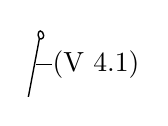
\begin{tikzpicture}[x=1cm,y=1cm,baseline=(ref.base)]
\draw[line width=.5pt] (0,-.22) -- (.14,.52);
\draw[line width=.5pt] (.14,.52) .. controls (.10,.58) and (.14,.65) .. (.18,.60) .. controls (.22,.54) and (.17,.50) .. (.14,.52);
\draw[line width=.4pt] (.10,.19) -- (.30,.19);
\node[anchor=west,inner sep=0pt] (ref) at (.30,.19) {\inserted{(V 4.1)}};
\end{tikzpicture}}}\normalmarginpar . Deduce from this that for every abelian sheaf \(F\) of \(S^{\handwritten{\sim}}_{\handwritten{/}X}\) and every integer \(q\) , the group \(H^q(X,F)\) (cohomology computed in \(S^{\handwritten{\sim}}_{\handwritten{/}X}\) ) is canonically isomorphic to the group \(H^q(X,\operatorname{Res}_X F)\) (cohomology computed in \(S(X)^{\handwritten{\sim}}\) ) .

\handwritten{6}) Deduce from 5) that for every abelian sheaf \(G\) \deleted{on} of \(S(X)^{\handwritten{\sim}}\) and every integer \(q\) the group \(H^q(X,G)\) \deleted{(resp.} (cohomology computed in \(S(X)^{\handwritten{\sim}}\) ) is canonically isomorphic to the groups \(H^q(X,f_{\handwritten{*}}G)\) and \(H^q(X,\operatorname{Prol}_X G)\) (cohomology computed in \(S^{\handwritten{\sim}}_{\handwritten{/}X}\) ) .
% archive sheet number: 10
